\documentclass[11pt]{article}

% ===================== PACKAGES =====================
\usepackage{fontspec}
\usepackage[margin=2.2cm]{geometry}
\usepackage{xcolor}
\usepackage{tcolorbox}
\tcbuselibrary{skins,breakable}
\usepackage{titlesec}
\usepackage{graphicx}
\usepackage{tikz}
\usetikzlibrary{positioning,arrows.meta,shapes.geometric}
\usepackage{enumitem}
\usepackage{fancyhdr}
\usepackage{longtable}
\usepackage{booktabs}
\usepackage{hyperref}
\usepackage{listings}

% ===================== COLORS =====================
\definecolor{navy}{HTML}{111827}
\definecolor{darknavy}{HTML}{0B1220}
\definecolor{teal}{HTML}{0F766E}
\definecolor{tealLight}{HTML}{E6F4F1}
\definecolor{amber}{HTML}{D97706}
\definecolor{amberLight}{HTML}{FEF3E2}
\definecolor{graytext}{HTML}{374151}
\definecolor{lightgray}{HTML}{F3F4F6}
\definecolor{bordergray}{HTML}{D1D5DB}
\definecolor{codebg}{HTML}{0D1117}
\definecolor{codefg}{HTML}{C9D1D9}

% ===================== FONTS =====================
\setmainfont{Latin Modern Roman}
\newfontfamily\headingfont{Latin Modern Roman}

% ===================== SECTION STYLE =====================
\titleformat{\section}
  {\Large\bfseries\color{navy}}
  {\thesection}{0.6em}{}
\titleformat{\subsection}
  {\large\bfseries\color{teal}}
  {\thesubsection}{0.5em}{}
\titlespacing*{\section}{0pt}{1.6em}{0.8em}

% ===================== CODE LISTING STYLE =====================
\lstdefinestyle{term}{
  backgroundcolor=\color{codebg},
  basicstyle=\ttfamily\scriptsize\color{codefg},
  breaklines=true,
  frame=single,
  rulecolor=\color{bordergray},
  framerule=0.4pt,
  columns=fullflexible,
  keepspaces=true,
  showstringspaces=false,
  xleftmargin=4pt,
  xrightmargin=4pt,
  aboveskip=6pt,
  belowskip=6pt
}
\lstset{style=term}

% ===================== HEADER/FOOTER =====================
\pagestyle{fancy}
\fancyhf{}
\renewcommand{\headrulewidth}{0.6pt}
\renewcommand{\headrule}{\hbox to\headwidth{\color{bordergray}\leaders\hrule height \headrulewidth\hfill}}
\fancyhead[L]{\small\color{graytext} AD Enumeration Report}
\fancyhead[R]{\small\color{graytext} DEPI -- Vulnerability Analyst \& Penetration Tester Track}
\fancyfoot[C]{\small\color{graytext}\thepage}

% ===================== CUSTOM BOXES =====================
\newtcolorbox{infobox}[1][]{
  colback=tealLight, colframe=teal, boxrule=0.8pt, arc=2pt,
  left=8pt, right=8pt, top=6pt, bottom=6pt, breakable, #1
}
\newtcolorbox{warnbox}[1][]{
  colback=amberLight, colframe=amber, boxrule=0.8pt, arc=2pt,
  left=8pt, right=8pt, top=6pt, bottom=6pt, breakable, #1
}
\newtcolorbox{sectionbox}[2][]{
  enhanced, breakable, colback=white, colframe=bordergray, boxrule=0.6pt, arc=3pt,
  fonttitle=\bfseries\color{white}, coltitle=white,
  colbacktitle=navy,
  title={#2}, left=8pt, right=8pt, top=6pt, bottom=6pt, #1
}
\newtcolorbox{evidencebox}[1][]{
  colback=lightgray, colframe=bordergray, boxrule=0.5pt, arc=2pt,
  left=6pt, right=6pt, top=6pt, bottom=6pt, breakable, #1
}

\newcommand{\evidence}[3]{%
  \begin{evidencebox}
    \textbf{\small\color{navy} Evidence: #1}\\[4pt]
    \begin{center}
      \includegraphics[width=#3\linewidth]{#2}
    \end{center}
  \end{evidencebox}
}

% ===================== TITLE PAGE =====================
\begin{document}

\begin{titlepage}
\centering
\vspace*{1.5cm}
{\color{teal}\rule{\linewidth}{2pt}}\\[0.6cm]
{\huge\bfseries\color{navy} Active Directory Enumeration Report}\\[0.4cm]
{\Large\color{graytext} AttacktiveDirectory Lab -- \texttt{spookysec.local}}\\[0.8cm]
{\color{teal}\rule{\linewidth}{2pt}}\\[1.5cm]

\begin{tabular}{ll}
\textbf{Prepared by:} & Eyad El-Taher \\
\textbf{Track:} & DEPI -- Vulnerability Analyst \& Penetration Tester \\
\textbf{Target Domain:} & spookysec.local (NetBIOS: THM-AD) \\
\textbf{Target Host:} & ATTACKTIVEDIREC (10.113.130.110) \\
\textbf{Engagement Type:} & Authorized Lab Enumeration \\
\textbf{Date:} & August 29--30, 2026 \\
\end{tabular}

\vfill

\begin{warnbox}
\textbf{Authorized Lab Environment Only.} All enumeration described in this
report was performed exclusively against the assigned lab environment. These
techniques translate directly to real production Active Directory environments --
written authorization must always be confirmed before enumerating any environment
not owned or managed by the tester.
\end{warnbox}

\end{titlepage}

\tableofcontents
\newpage

% =====================================================
\section{Domain Information}
% =====================================================
\begin{sectionbox}{Summary}
\begin{tabular}{@{}ll}
\textbf{Domain (FQDN):} & spookysec.local \\
\textbf{NetBIOS Domain Name:} & THM-AD \\
\textbf{Domain SID:} & S-1-5-21-3591857110-2884097990-301047963 \\
\textbf{Forest Context:} & Single-domain forest, no external/incoming trusts \\
\textbf{Namespace:} & spookysec.local (also resolves as AttacktiveDirectory.spookysec.local) \\
\textbf{Functional Level Indicator:} & msDS-Behavior-Version: 7 (Windows Server 2016 domain mode) \\
\end{tabular}
\end{sectionbox}

\vspace{0.4cm}
Domain trust enumeration via \texttt{ldapdomaindump} returned an empty result set,
confirming the domain operates as an isolated forest root with no configured
incoming or outgoing trusts.

\evidence{Nmap service scan identifying the domain and core AD services}{img/command6.png}{0.95}

% =====================================================
\section{Domain Controllers}
% =====================================================
\begin{sectionbox}{Domain Controller Identified}
\begin{tabular}{@{}ll}
\textbf{Hostname:} & ATTACKTIVEDIREC \\
\textbf{FQDN:} & AttacktiveDirectory.spookysec.local \\
\textbf{IP Address:} & 10.113.130.110 (later re-observed as 10.114.176.243 / 10.114.156.161) \\
\textbf{Operating System:} & Windows Server 2019 Standard, Build 17763 \\
\textbf{Role:} & Sole Domain Controller (OU=Domain Controllers) \\
\textbf{FSMO Role Owner:} & ATTACKTIVEDIREC (NTDS Settings) -- holds all FSMO roles \\
\end{tabular}
\end{sectionbox}

\vspace{0.3cm}
Only a single domain controller was identified in this environment, meaning it holds
every FSMO role (Schema Master, Domain Naming Master, RID Master, PDC Emulator, and
Infrastructure Master) by default. Key open services confirming its DC role: LDAP
(389/3268), Kerberos (88), \texttt{kpasswd} (464), and SMB/RPC (135/139/445).

\evidence{Full Nmap port/service scan of the domain controller}{img/command6.png}{0.95}

% =====================================================
\section{Users Discovered}
% =====================================================
\begin{sectionbox}{Enumeration Methods Used}
\begin{itemize}[leftmargin=1.2em]
  \item \texttt{enum4linux} -- RID cycling over a null SMB session (RIDs 500--550, 1000--1050)
  \item \texttt{kerbrute userenum} -- Kerberos pre-authentication username validation (73{,}317 candidates tested, 16 valid)
  \item \texttt{netexec (nxc) smb --users} -- authenticated SAM enumeration once Administrator hash was obtained
\end{itemize}
\end{sectionbox}

\vspace{0.3cm}
\textbf{17 domain accounts} (16 standard/service + built-in Administrator/Guest/krbtgt)
were enumerated in total:

\begin{center}
\begin{tabular}{@{}ll@{\hspace{2cm}}ll@{}}
\toprule
\textbf{Account} & \textbf{Type} & \textbf{Account} & \textbf{Type} \\
\midrule
Administrator & Built-in / Domain Admin & darkstar & Standard (CompStaff) \\
Guest & Built-in (disabled) & Ori & Standard (CompStaff) \\
krbtgt & KDC service account & robin & Standard (CompStaff) \\
skidy & Standard (CompStaff) & paradox & Standard (CompStaff) \\
breakerofthings & Standard (CompStaff) & Muirland & Standard (CompStaff) \\
james & Standard (CompStaff) & horshark & Standard (CompStaff) \\
optional & Standard (CompStaff) & svc-admin & Service account (CompStaff) \\
sherlocksec & Standard (CompStaff) & backup & Standard (no group) \\
a-spooks & \multicolumn{3}{l}{Privileged -- Domain Admins \& Enterprise Admins} \\
\bottomrule
\end{tabular}
\end{center}

\textbf{Administrative accounts of note:} \texttt{svc-admin} (service account, vulnerable
to AS-REP roasting) and \texttt{backup} (holder of leaked credentials, see Section~9)
were the two accounts leading directly to full compromise.

\evidence{Kerberos pre-authentication username enumeration with kerbrute}{img/command3.png}{0.95}
\evidence{RID cycling via enum4linux revealing domain users and groups}{img/command2.png}{0.95}
\evidence{Authenticated SAM user listing via netexec}{img/command11.png}{0.95}

% =====================================================
\section{Groups Identified}
% =====================================================
\begin{sectionbox}{Notable Security \& Administrative Groups}
\begin{tabular}{@{}lll}
\textbf{Group} & \textbf{Members} & \textbf{Description} \\
\midrule
Domain Admins & 2 & Designated administrators of the domain \\
Enterprise Admins & 2 & Designated administrators of the enterprise \\
Schema Admins & 1 & Designated administrators of the schema \\
Administrators (Builtin) & 3 & Complete/unrestricted access to the computer/domain \\
Remote Desktop Users & 4 & Granted right to log on remotely \\
Backup Operators & 0 & Can override security restrictions for backup/restore \\
Group Policy Creator Owners & 1 & Can modify Group Policy for the domain \\
CompStaff & 12 & Custom group holding the majority of standard users \\
DnsAdmins & 0 & DNS Administrators group \\
\end{tabular}
\end{sectionbox}

\vspace{0.3cm}
A total of 54 groups were enumerated via \texttt{bloodhound-python}, of which the LDAP
group query above surfaced the built-in privileged groups plus one custom
organizational group, \textbf{CompStaff}, used to bulk-assign standard employee
accounts. No nested/non-standard group memberships beyond the expected Domain
Admins $\rightarrow$ Administrators nesting were identified.

\evidence{LDAP group enumeration via netexec, including membership counts}{img/command12.png}{0.95}

% =====================================================
\section{Privileged Accounts}
% =====================================================
\begin{warnbox}
\textbf{Domain/Enterprise Admins identified:} \texttt{Administrator} and \texttt{a-spooks}
are both members of \textbf{Domain Admins} and \textbf{Enterprise Admins}. The
\texttt{Administrator} account is additionally a member of \textbf{Schema Admins} and
\textbf{Group Policy Creator Owners}, giving it forest-wide schema modification rights
in addition to domain-wide administrative control.
\end{warnbox}

\begin{center}
\begin{tabular}{@{}lll}
\toprule
\textbf{Account} & \textbf{Privileged Group Membership} & \textbf{Notes} \\
\midrule
Administrator & Domain Admins, Enterprise Admins, & Built-in administrator; \\
 & Schema Admins, GPO Creator Owners & final compromised account \\
a-spooks & Domain Admins, Enterprise Admins & Secondary highly-privileged account \\
svc-admin & Standard user (CompStaff) & Not privileged, but AS-REP roastable -- \\
 & & used as the initial foothold \\
backup & No group membership & Held leaked domain credentials \\
\bottomrule
\end{tabular}
\end{center}

Neither \texttt{svc-admin} nor \texttt{backup} are privileged accounts by group
membership; their value lay in credential exposure, which was pivoted into full
Domain Admin compromise via \texttt{secretsdump.py} (NTDS.DIT extraction) once
\texttt{backup}'s DRSUAPI replication rights were leveraged.

% =====================================================
\section{Service Accounts}
% =====================================================
\begin{sectionbox}{Service / Application Accounts}
\begin{itemize}[leftmargin=1.2em]
  \item \textbf{svc-admin} -- naming convention and behavior (\texttt{UF\_DONT\_REQUIRE\_PREAUTH}
        not initially visible, but AS-REP roastable) indicate a service account used for
        administrative automation. Cracked password: \texttt{management2005}.
  \item \textbf{krbtgt} -- built-in Key Distribution Center service account; keys
        recovered post-compromise via \texttt{secretsdump.py} for completeness
        (Kerberos ticket-forging awareness).
  \item \textbf{ATTACKTIVEDIREC\$} -- the machine account of the domain controller
        itself, enumerated as part of the computer object.
\end{itemize}
No standalone Managed Service Accounts (MSAs/gMSAs) were present in the directory.
\end{sectionbox}

\evidence{AS-REP roasting against svc-admin yielding a crackable krb5asrep hash}{img/command5.png}{0.95}
\evidence{Cracking the AS-REP hash offline with hashcat (mode 18200)}{img/command4.png}{0.95}

% =====================================================
\section{Shared Resources}
% =====================================================
\begin{center}
\begin{tabular}{@{}llll}
\toprule
\textbf{Share} & \textbf{Type} & \textbf{Access Level (as Administrator)} & \textbf{Notes} \\
\midrule
ADMIN\$ & DISK (SPECIAL) & READ, WRITE & Remote admin; used by psexec.py for shell access \\
C\$ & DISK (SPECIAL) & READ, WRITE & Default administrative share \\
IPC\$ & IPC (SPECIAL) & READ & Remote IPC \\
NETLOGON & DISK & READ, WRITE & Logon server share \\
SYSVOL & DISK & READ, WRITE & Logon server share (GPO storage) \\
backup & DISK & WRITE (ACL) & Contained \texttt{backup\_credentials.txt} \\
\bottomrule
\end{tabular}
\end{center}

\begin{infobox}
The \textbf{backup} share was accessible via a null/unauthenticated SMB session and
contained a plaintext file, \texttt{backup\_credentials.txt}, holding a Base64-encoded
credential pair: \texttt{backup@spookysec.local:backup2517860}. This was the pivot point
from an unprivileged foothold to domain credential extraction.
\end{infobox}

\evidence{Anonymous access to the backup share revealing backup\_credentials.txt}{img/command7.png}{0.95}
\evidence{Share and permission enumeration as Administrator via netexec}{img/command13.png}{0.95}

% =====================================================
\section{Key Relationships}
% =====================================================
\begin{center}
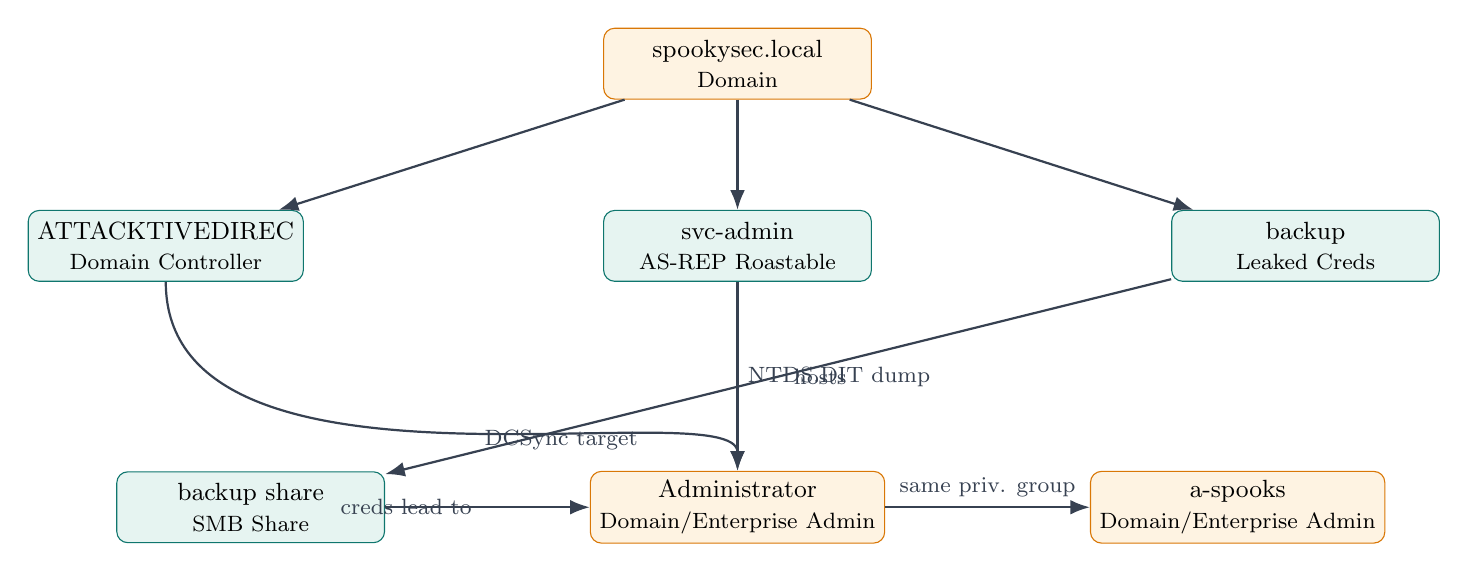
\begin{tikzpicture}[
  node distance=1.4cm and 2.6cm,
  every node/.style={font=\small},
  box/.style={draw, rounded corners, fill=tealLight, draw=teal, minimum width=3.4cm, minimum height=0.9cm, align=center},
  boxadmin/.style={draw, rounded corners, fill=amberLight, draw=amber, minimum width=3.4cm, minimum height=0.9cm, align=center},
  arr/.style={-{Latex[length=2.5mm]}, thick, color=graytext}
]

\node[boxadmin] (dom) {spookysec.local\\\footnotesize Domain};
\node[box, below left=of dom, xshift=-1.2cm] (dc) {ATTACKTIVEDIREC\\\footnotesize Domain Controller};
\node[box, below=of dom] (svc) {svc-admin\\\footnotesize AS-REP Roastable};
\node[box, below right=of dom, xshift=1.2cm] (backup) {backup\\\footnotesize Leaked Creds};
\node[boxadmin, below=2.4cm of svc] (admin) {Administrator\\\footnotesize Domain/Enterprise Admin};
\node[boxadmin, right=of admin] (aspooks) {a-spooks\\\footnotesize Domain/Enterprise Admin};
\node[box, left=of admin] (share) {backup share\\\footnotesize SMB Share};

\draw[arr] (dom) -- (dc);
\draw[arr] (dom) -- (svc);
\draw[arr] (dom) -- (backup);
\draw[arr] (backup) -- (share) node[midway, right, xshift=2pt]{\footnotesize hosts};
\draw[arr] (share) -- (admin) node[midway, left, xshift=-2pt]{\footnotesize creds lead to};
\draw[arr] (svc) .. controls +(down:1.2cm) and +(up:1.2cm) .. (admin) node[midway, right]{\footnotesize NTDS.DIT dump};
\draw[arr] (admin) -- (aspooks) node[midway, above]{\footnotesize same priv. group};
\draw[arr] (dc) .. controls +(down:3.5cm) and +(up:1.5cm) .. (admin) node[near end, left]{\footnotesize DCSync target};

\end{tikzpicture}
\end{center}

\begin{infobox}
\textbf{Relationship narrative:} The \texttt{backup} share (anonymously readable)
exposed credentials for the \texttt{backup} user, which -- combined with the
\texttt{svc-admin} account's AS-REP roastable password (\texttt{management2005}) --
enabled a DCSync-style secrets dump of the entire NTDS.DIT via
\texttt{secretsdump.py}, yielding the \texttt{Administrator} NTLM hash and full
domain compromise. \texttt{Administrator} and \texttt{a-spooks} share identical
Domain/Enterprise Admin privileges.
\end{infobox}

\evidence{BloodHound relationship graph of the spookysec.local domain}{img/bloodhound.png}{0.85}

\newpage
% =====================================================
\section{Security Observations}
% =====================================================
\begin{sectionbox}{Findings}
\begin{enumerate}[leftmargin=1.4em]
  \item \textbf{Null/anonymous SMB sessions permitted} -- allowed full RID cycling,
        user enumeration, and read access to the \texttt{backup} share without any
        credentials.
  \item \textbf{Plaintext credentials stored on an SMB share} -- \texttt{backup\_credentials.txt}
        contained a Base64-encoded (trivially reversible) username/password pair.
  \item \textbf{AS-REP roasting exposure} -- \texttt{svc-admin} was crackable offline
        via Kerberos pre-authentication weaknesses, and its password
        (\texttt{management2005}) was present in the \texttt{rockyou.txt} wordlist.
  \item \textbf{Weak/reused password policy indicators} -- minimum password length
        of \texttt{0} configured in the domain password policy (\texttt{minPwdLength: 0}).
  \item \textbf{Excessive replication rights} -- the compromised account chain
        permitted a full DRSUAPI-based NTDS.DIT extraction (\texttt{secretsdump.py}),
        equivalent to a DCSync attack, from a non-Domain-Admin foothold.
  \item \textbf{Single point of failure} -- only one domain controller exists,
        holding all FSMO roles with no redundancy.
\end{enumerate}
\end{sectionbox}

\evidence{Full NTDS.DIT secrets dump via the DRSUAPI method}{img/command8.png}{0.95}
\evidence{Post-compromise interactive shell via psexec.py using the Administrator hash}{img/command10.png}{0.95}

% =====================================================
\section{Recommendations}
% =====================================================
\begin{sectionbox}{Hardening Suggestions}
\begin{enumerate}[leftmargin=1.4em]
  \item Disable anonymous/null SMB sessions (\texttt{RestrictAnonymous} = 2) to
        prevent unauthenticated RID cycling and share enumeration.
  \item Remove world-readable/writable SMB shares containing credentials; enforce
        least-privilege ACLs and never store plaintext or Base64-"obfuscated"
        secrets on file shares.
  \item Enable \texttt{UF\_DONT\_REQUIRE\_PREAUTH}-aware monitoring and enforce Kerberos
        pre-authentication for all service accounts to mitigate AS-REP roasting.
  \item Enforce a strong password policy: raise \texttt{minPwdLength} well above 0
        (14+ characters recommended), enable complexity requirements, and rotate
        service account passwords regularly.
  \item Restrict directory replication rights (\texttt{Replicating Directory Changes} /
        \texttt{Replicating Directory Changes All}) to only Domain Controllers and
        explicitly authorized tier-0 accounts to prevent DCSync-style attacks.
  \item Deploy a secondary domain controller for redundancy and to distribute
        FSMO roles/reduce single-point-of-failure risk.
  \item Monitor for Kerberoasting/AS-REP roasting activity via SIEM detections on
        excessive TGT/TGS requests for service accounts.
\end{enumerate}
\end{sectionbox}

\vspace{1cm}
\begin{center}
{\small\color{graytext} -- End of Report --}
\end{center}

\end{document}
